\documentclass{sig-alternate-ipsn13}
\usepackage{graphicx}

\begin{document}

\title{WiP Abstract: Preliminary Evaluation for ROS2}
% Format\titlenote{(Does NOT produce the permission block, copyright information nor page numbering). Supported by ACM.}}
%
% You need the command \numberofauthors to handle the 'placement
% and alignment' of the authors beneath the title.
%
% For aesthetic reasons, we recommend 'three authors at a time'
% i.e. three 'name/affiliation blocks' be placed beneRath the title.
%
% NOTE: You are NOT restricted in how many 'rows' of
% "name/affiliations" may appear. We just ask that you restrict
% the number of 'columns' to three.
%
% Because of the available 'opening page real-estate'
% we ask you to refrain from putting more than six authors
% (two rows with three columns) beneath the article title.
% More than six makes the first-page appear very cluttered indeed.
%
% Use the \alignauthor commands to handle the names
% and affiliations for an 'aesthetic maximum' of six authors.
% Add names, affiliations, addresses for
% the seventh etc. author(s) as the argument for the
% \additionalauthors command.
% These 'additional authors' will be output/set for you
% without further effort on your part as the last section in
% the body of your article BEFORE References or any Appendices.

\numberofauthors{3} %  in this sample file, there are a *total*
% of EIGHT authors. SIX appear on the 'first-page' (for formatting
% reasons) and the remaining two appear in the \additionalauthors section.
%
\author{
% You can go ahead and credit any number of authors here,
% e.g. one 'row of three' or two rows (consisting of one row of three
% and a second row of one, two or three).
%
% The command \alignauthor (no curly braces needed) should
% precede each author name, affiliation/snail-mail address and
% e-mail address. Additionally, tag each line of
% affiliation/address with \affaddr, and tag the
% e-mail address with \email.
%
% 1st. author
\alignauthor Yuya Maruyama\\
\affaddr{School of Engineering Science}\\
\affaddr{Osaka University}\\
       % \affaddr{Institute for Clarity in Documentation}\\
       % \affaddr{1932 Wallamaloo Lane}\\
       % \affaddr{Wallamaloo, New Zealand}\\
       % \email{trovato@corporation.com}
% 2nd. author
\alignauthor Shinpei Kato\\
\affaddr{Graduate School of Information Science}\\
\affaddr{Nagoya University}\\
       % \affaddr{Institute for Clarity in Documentation}\\
       % \affaddr{P.O. Box 1212}\\
       % \affaddr{Dublin, Ohio 43017-6221}\\
       % \email{webmaster@marysville-ohio.com}
% 3rd. author
\alignauthor Takuya Azumi\\
\affaddr{Graduate School of Engineering Science}\\
\affaddr{Osaka University}\\
       % \affaddr{The Th{\o}rv{\"a}ld Group}\\
       % \affaddr{1 Th{\o}rv{\"a}ld Circle}\\
       % \affaddr{Hekla, Iceland}\\
       % \email{larst@affiliation.org}
% \and  % use '\and' if you need 'another row' of author names
% % 4th. author
% \alignauthor Lawrence P. Leipuner\\
%        \affaddr{Brookhaven Laboratories}\\
%        \affaddr{Brookhaven National Lab}\\
%        \affaddr{P.O. Box 5000}\\
%        \email{lleipuner@researchlabs.org}
% % 5th. author
% \alignauthor Sean Fogarty\\
%        \affaddr{NASA Ames Research Center}\\
%        \affaddr{Moffett Field}\\
%        \affaddr{California 94035}\\
%        \email{fogartys@amesres.org}
% % 6th. author
% \alignauthor Charles Palmer\\
%        \affaddr{Palmer Research Laboratories}\\
%        \affaddr{8600 Datapoint Drive}\\
%        \affaddr{San Antonio, Texas 78229}\\
%        \email{cpalmer@prl.com}
}
% There's nothing stopping you putting the seventh, eighth, etc.
% author on the opening page (as the 'third row') but we ask,
% for aesthetic reasons that you place these 'additional authors'
% in the \additional authors block, viz.
% \additionalauthors{Additional authors: John Smith (The Th{\o}rv{\"a}ld Group,
% email: {\texttt{jsmith@affiliation.org}}) and Julius P.~Kumquat
% (The Kumquat Consortium, email: {\texttt{jpkumquat@consortium.net}}).}
% \date{30 July 1999}
% Just remember to make sure that the TOTAL number of authors
% is the number that will appear on the first page PLUS the
% number that will appear in the \additionalauthors section.

\maketitle
% \begin{abstract}

% \end{abstract}

% \section{Introduction}

Cyber-Physical Systems (CPS) represent next generation distributed and embedded systems. Becoming complicated and diverse, CPS applications aim to monitor and control complex real-time phenomena. Robot Operating System (ROS), an open-source middleware for robotics development, has been widely used for CPS applications (e.g. an autonomous car). ROS provides a Publish/Subscribe transport, many libraries (e.g. Point Cloud Library), and tools to help software-developers create CPS applications.

However, ROS does not support to meet real-time requirements and runs only on a few kinds of OSs. Therefore, ROS is not suitable for real-time and embedded systems. Facing this problem, ROS is going to be significantly upgraded as ROS2 \cite{ros2_iccps2016}. ROS2 considers following use cases: real-time systems, non-ideal networks, small embedded systems, and cross-platform.

Existing ROS (hereinafter referred to as ROS1) reached the time to be reconstructed with improving user interfacing APIs and utilizing new technologies (e.g. Data Distribution Service (DDS) \cite{pardo2003omg}). Replacing the ROS1's transport system, DDS is an industry-standard real-time communication system as end-to-end middleware that provides reliable Publish/Subscribe transport.

The next generation communication system of ROS, DDS, is suitable for CPS due to its various transport configurations such as DEADLINE, RELIABILITY, and DURABILITY. It has multiple implementations; some small/embedded solutions reduce their library size and memory footprints. Developed by different DDS vendors, several implementations are used in mission-critical environments and verified by NASA. Therefore, ROS2 built on DDS obtains its reliability and flexibility.

Figure \ref{fig:graph} shows data communication time between nodes on ROS1 or ROS2. ROS2 using DDS has various transport configurations, which causes the overhead examined in this research. ROS2 needs to convert data for DDS and abstracting DDS from ROS2 users. The overhead contains these transactions and the difference between ROS1 communication system and DDS. These influence varies by transport situations, data size, and DDS vendors.

In this research, we clarify the performance characteristics of currently-available data transport between nodes on ROS1 or ROS2 in various situations. Revealing the present capability of ROS2 depending on DDS vendors and DDS configurations, we explore and evaluate the facing constraints and potential of ROS2. The advantage and disadvantage of the current ROS2 are clarified with problems in the case ROS1 and ROS2 coexist. To the best of our knowledge, this evaluation is the first work for exploring the performance of ROS2.

% \begin{figure}[t]
% \begin{center}
% \includegraphics{fly.eps}
% \caption{A sample black and white graphic (.eps format).}
% \label{fig:example}
% \end{figure}

% \begin{figure}[t]
% \begin{center}
% 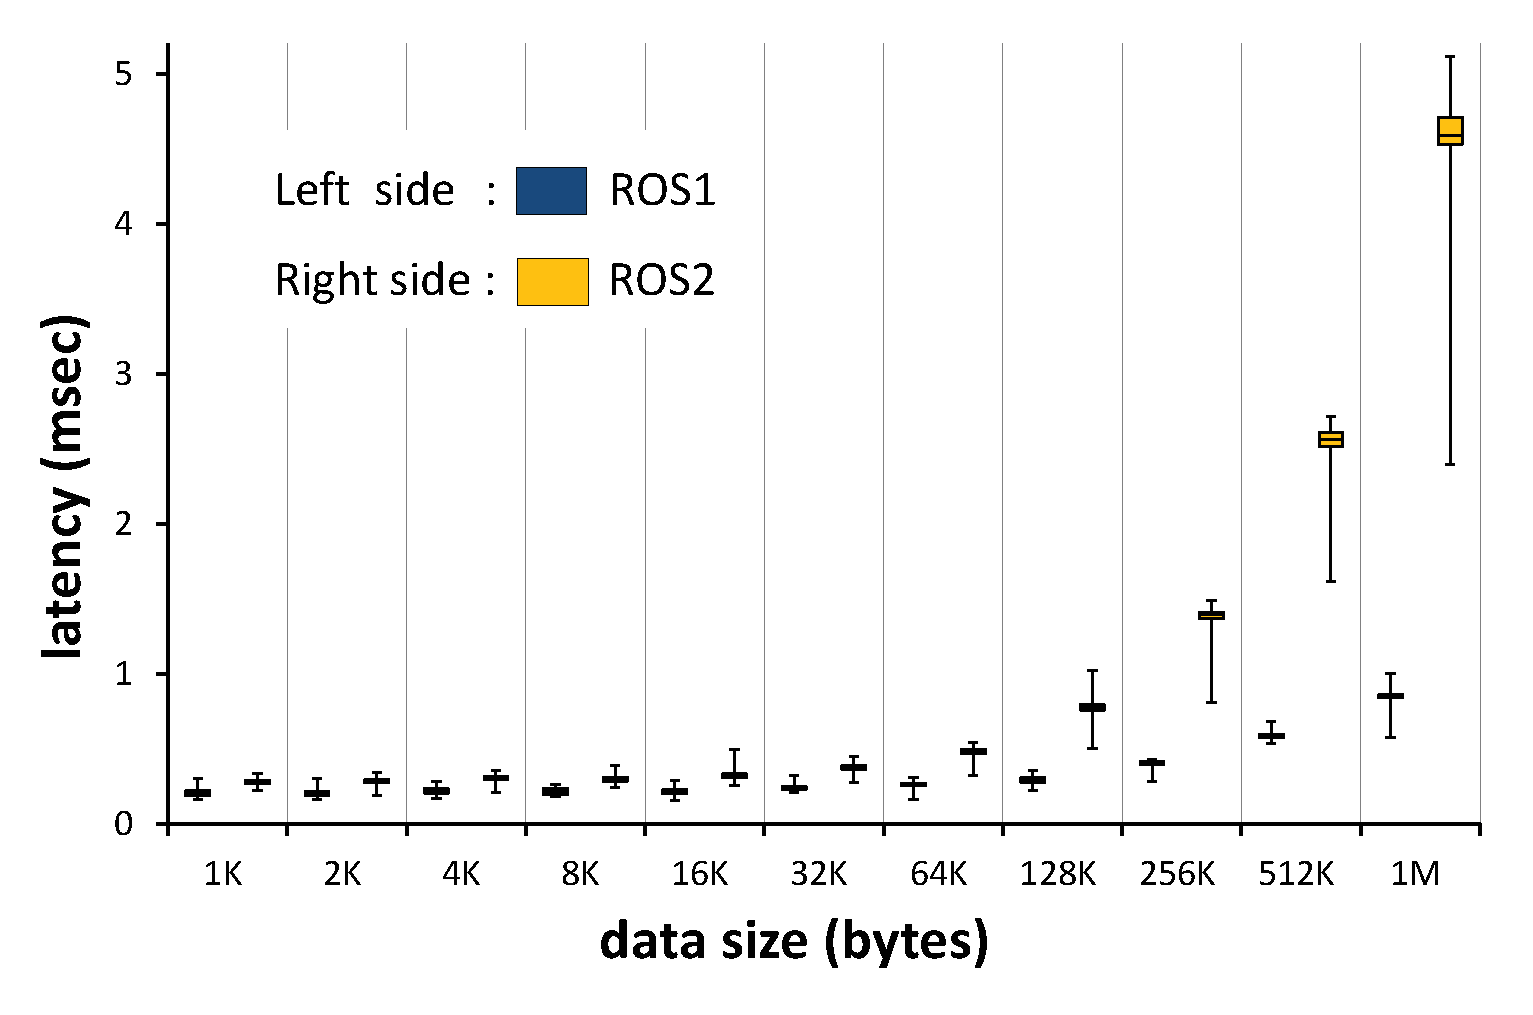
\includegraphics{graph.eps}
% \caption{A sample black and white graphic (.eps format).}
% \label{fig:example}
% \end{figure}

\begin{figure}[t]
\begin{center}
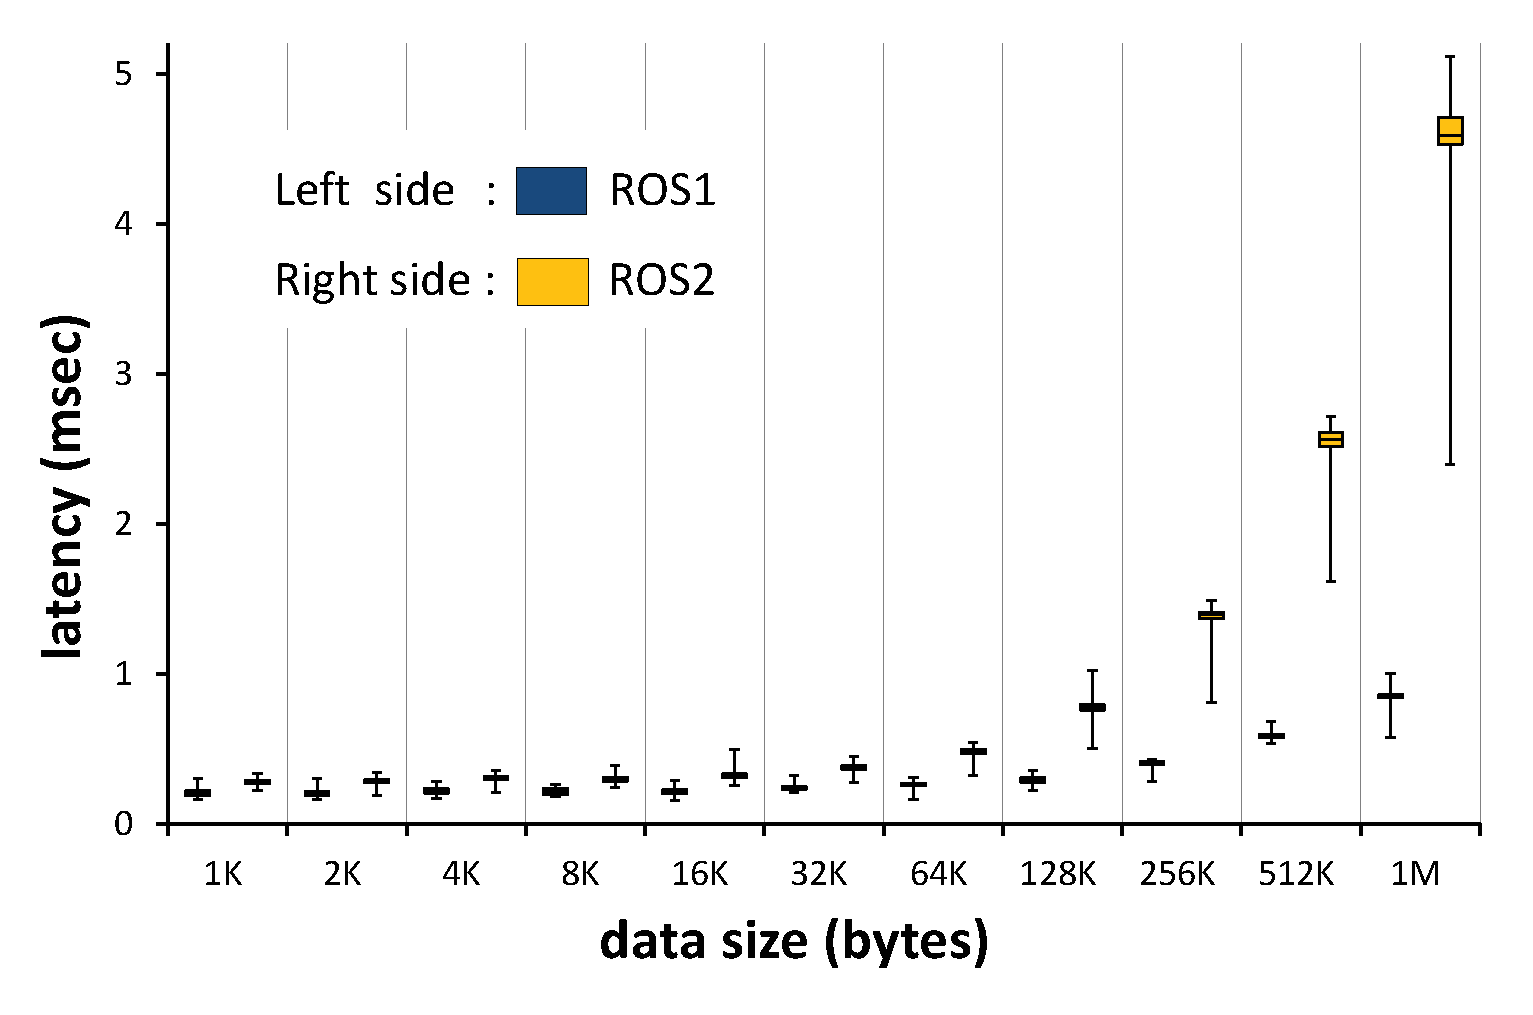
\includegraphics[scale=0.33]{graph.eps}
%\epsfig{file=sys_config_2.eps, width=80mm}
\end{center}
\vspace{-8.mm}
\caption{Comparison of transport latency variation in ROS1 or ROS2}
\vspace{-5.0mm}
\label{fig:graph}
\end{figure}

% \section{Conclusions}
% Conclusion goes here.

%ACKNOWLEDGMENTS are optional
% \section*{Acknowledgments}
% Acknowledgement goes here.

%
% The following two commands are all you need in the
% initial runs of your .tex file to
% produce the bibliography for the citations in your paper.
% \bibliography{sigproc}  % sigproc.bib is the name of the Bibliography in this case
\vspace{-3.0mm}
\bibliographystyle{abbrv}
\bibliography{reference}

% You must have a proper ".bib" file
%  and remember to run:
% latex bibtex latex latex
% to resolve all references
%
% ACM needs 'a single self-contained file'!
%
%APPENDICES are optional
%\balancecolumns
% \appendix
% %Appendix A

% Appendix goes here.

% That's all folks!
\end{document}
